\chapter{Kvantově inspirované evoluční algoritmy} \label{chapt:qiea}
Algoritmy, které vycházejí z principů kvantové mechaniky se souhrnně označují jako kvantově inspirované evoluční algoritmy (\emph{Quantum Inspired Evolutionary Algorithms\,--\,QIEA}) a jsou aplikovány na optimalizační problémy. 
Není možné, aby tyto algoritmy využívaly všechny náležitosti vyplývající z kvantové mechaniky. 
Jedná se zejména o kvantové provázání, které nelze efektivně simulovat na klasických počítačích. 
Nicméně použití v evolučních algoritmech kvantově inspirované reprezentace zaručuje dobrý kompromis mezi průzkumem a exploatací a to často při použití menší populace jedinců, než by bylo třeba při použití klasických evolučních algoritmů~\cite{NaturalComputing}.

Tato kapitola nejdříve popíše, jak lze reprezentovat jedince v populaci, a následně se zaměří na dva způsoby jejich manipulace. 
Posléze charakterizuje kvantově inspirovaný genetický algoritmus (\emph{Quantum Inspired Genetic Algorithm\,--\,QIGA}) a v poslední řadě souhrnně vylíčí zajímavé studie popisující situace, kde byly QIEA využity. 

\section{Kódování řešení v kvantově inspirovaných evolučních algoritmech}
Jeden z možných způsobů reprezentace jedince v populaci v kvantově inspirovaných evolučních algoritmech vychází z konceptu kvantového bitu. 
Binární kvantově inspirované evoluční algoritmy využívají qubity k reprezentaci řešení, přičemž manipulace s nimi probíhá prostřednictvím kvantově inspirovaných operátorů.

V binárním kvantově inspirovaném evolučním algoritmu je qubit popsán dvojicí koeficientů $\alpha$ a~$\beta$, přičemž systém sestávající z $m$ qubitů lze zapsat v podobě matice jako: 
\begin{equation}\label{eq:quantum-representation}
    \begin{bmatrix}
        \alpha_1 & \alpha_2 & \dots & \alpha_m \\
        \beta_1  & \beta_2  & \dots & \beta_m
    \end{bmatrix},
\end{equation}
přičemž v případě normalizovaného systému musí platit:
\begin{equation}\label{eq:normalized-quantum-representation}
    \forall i \in \left\{1,2,\dots,m \right\}: \alpha^2_i + \beta^2_i = 1.
\end{equation}

Tento způsob umožňuje efektivní zápis qubitů, ale je však důležité si uvědomit, že kvantový systém o $m$ qubitech dokáže současně reprezentovat všechny bitové řetězce o~délce $2^m$ bitů, zatímco klasický bitový registr umožňuje reprezentovat pouze jeden z $2^m$ možných stavů~\cite{NaturalComputing}. 

Binární kvantově inspirované evoluční algoritmy využívají kvantovou reprezentaci, viz rovnici~\ref{eq:quantum-representation}, k reprezentaci pravděpodobnosti jednotlivých řešení. 
V případě splnění podmínky normalizace~\ref{eq:normalized-quantum-representation}, hodnota $\alpha^2_i$, respektive $\beta^2_i$, určuje s jakou pravděpodobností bude ve výsledném řetězci na $i$-té pozici binární hodnota $0$, respektive $1$, s ohledem k rovnici~\ref{eq:psi=a0+b1}.

\section{Operátory v kvantově inspirovaných algoritmech}
Pro generování diverzity populace se běžně využívají dva přístupy popsané níže, přičemž se nevyužívají klasické operátory křížení a mutace~\cite{NaturalComputing}.

\subsection{Kvantová hradla}
V kvantových systémech se s qubity manipuluje pomocí hradel (Hadamardovo, CNOT, Pauli-X,~aj.). 
Tyto hradla umožňují provádět paralelní výpočet nad všemi qubity najednou bez změření jejich hodnoty, přičemž jejich výstupem je nová superpozice systému~\cite{NaturalComputing,QuantumComputing-Curious,QuantumComputing-QuantumInformation}. 

V kvantově inspirovaných evolučních algoritmech našly kvantové brány uplatnění, kde rotační hradlo~\ref{eq:rotate-gate} je jedním z možných příkladů.
\begin{equation}\label{eq:rotate-gate}
    \begin{bmatrix}
        \cos{\left( \Delta\theta_i \right)} & - \sin{\left( \Delta\theta_i \right)} \\
        \sin{\left( \Delta\theta_i \right)} &   \cos{\left( \Delta\theta_i \right)}
    \end{bmatrix}
\end{equation}
Pravděpodobnostní koeficienty $\alpha_i$ a $\beta_i$ $i$-tých qubitů v chromozomu jsou modifikovány na nové koeficienty $\alpha_i'$ a $\beta_i'$ pomocí kvantové rotační brány~\ref{eq:rotate-gate} podle vzorce: 
\begin{equation}\label{eq:rotation-gate-angles}
    \begin{bmatrix}
        \alpha_i' \\
        \beta_i' 
    \end{bmatrix}
    =
    \begin{bmatrix}
        \cos{\left( \Delta\theta_i \right)} & - \sin{\left( \Delta\theta_i \right)} \\
        \sin{\left( \Delta\theta_i \right)} &   \cos{\left( \Delta\theta_i \right)}
    \end{bmatrix}
    \begin{bmatrix}
        \alpha_i \\
        \beta_i 
    \end{bmatrix},
\end{equation}
přičemž výsledné nové koeficienty musí splňovat podmínku normalizace~\ref{eq:a2+b2=1}. 
Tato podmínka je vždy splněna, jelikož kvantová rotační brána odpovídá unitární matici. 
\begin{figure}[ht!]
    \centering
    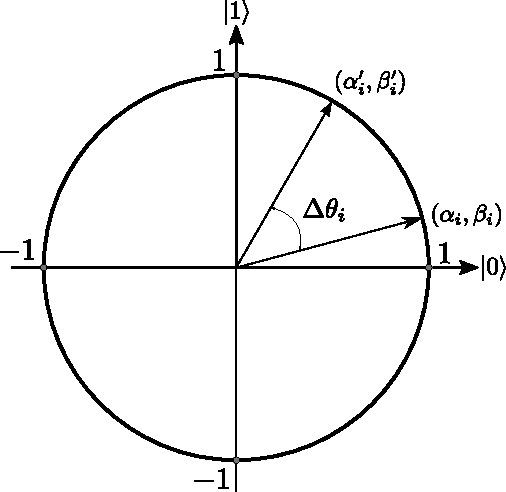
\includegraphics[width=0.45\textwidth]{rotation-gate.pdf}
    \caption{Kvantové rotační hradlo. Obrázek byl převzat s úpravami z~\cite{NaturalComputing}.}
    \label{fig:rotation-gate}
\end{figure}
Unitární vlastnost rotačního hradla zaručuje, že součet pravděpodobnosti bitového stavu $0$ a $1$ po pozorování zůstává roven $1$. 
Výsledný stav qubitu se tak po aplikaci hradla vždy nachází na jednotkové kružnici, viz obrázek~\ref{fig:rotation-gate}.

Aby mutace postupně přizpůsobovala hodnoty kvantového chromozomu směrem k nejlepšímu nalezenému jedinci v aktuální populaci, lze využít různé přístupy. 
Jeden z možných způsobů spočívá ve využití tabulky~\ref{tab:look-up-table-Delta}, kde postup pro výběr hodnoty parametru $\Delta\theta_i$ je následující~\cite{NaturalComputing}:
\begin{enumerate}
    \item Pomocí aktuálního kvantového chromozomu $q = \begin{pmatrix} q_1 & q_2 & \dots & q_m \end{pmatrix}$ složeného z kvantových bitů $ q_i = \left( \alpha_i, \beta_i \right)$ pro $1,2,\dots,m$, respektive
        \begin{equation*}
            q =
            \begin{bmatrix}
                \alpha_1 & \alpha_2 & \dots & \alpha_m \\
                \beta_1  & \beta_2  & \dots & \beta_m
            \end{bmatrix},
        \end{equation*}
        je vytvořen binární chromozom $x = \begin{pmatrix} x_1 & x_2 & \dots & x_m \end{pmatrix}$.
        Hodnota $x_i$ je určena na základě qubitu $q_i$, respektive jeho parametru $\alpha_i$,~následovně:
        \begin{equation*}
            x_i =
            \begin{cases} 
                0 & \text{pokud } \alpha_i \leq 0.5, \\
                1 & \text{jinak}.
            \end{cases}
        \end{equation*}
    \item Z populace je vybráno nejlepší binární řešení $b = \begin{pmatrix} b_1 & b_2 & \dots & b_m \end{pmatrix}$.
    \item Na základě hodnot $x_i$ a $b_i$ je z vyhledávací tabulky~\ref{tab:look-up-table-Delta} vybrána hodnota $\Delta\theta_i$ následovně:
        \begin{table}[ht!]
            \centering
            \begin{tabular}{c c|c}
            \toprule
            \multicolumn{1}{c}{$x_i$} & \multicolumn{1}{c}{$b_i$} & \multicolumn{1}{|c}{$\Delta\theta_i$} \\
            \midrule
            1                       & 1                      & 0                      \\ 
            0                       & 1                      & $a$                      \\ 
            0                       & 0                      & 0                      \\ 
            1                       & 0                      & $-a$                     \\
            \bottomrule
            \end{tabular}
            \caption{Vyhledávací tabulka pro parametr $\Delta\theta$.}
            \label{tab:look-up-table-Delta}
        \end{table}
        \begin{itemize}
            \item Pokud $x_i = b_i$, pak $\Delta \theta = 0$, respektive parametry $\alpha_i$ a $\beta_i$ qubitu $q_i$ zůstanou zachovány.
            \item Pokud $x_i = 1 \wedge b_i = 0$, pak $\Delta \theta = -a$, respektive dojde ke snížení pravděpodobnosti pozorování binární hodnoty 1 na pozici $i$ chromozomu $q$. 
            \item Pokud $x_i = 0 \wedge b_i = 1$, pak $\Delta \theta =  a$, respektive dojde ke zvýšení pravděpodobnosti pozorování binární hodnoty 1 na pozici $i$ chromozomu $q$. 
        \end{itemize}
\end{enumerate}

V kvantově inspirovaných evolučních algoritmech se v současné době nevyužívají komplexní koeficienty z kvantové mechaniky, ale výlučně se používají reálné koeficienty, jak je vidět na obrázku~\ref{fig:rotation-gate}~\cite{NaturalComputing}.

\newpage
\subsection{Kvantová mutace}
Kvantová mutace se inspiruje mutací ze standardních genetických algoritmů v podobě:
\begin{equation*}
    Q^*(t) = a \times B_{best}(t) + (1 - a) * (1 - B_{best}(t))
\end{equation*}
\begin{equation*}
    Q(t+1) = Q^*(t) + b \times r,
\end{equation*}
kde
\begin{itemize}
    \item $B_{best}(t)$ reprezentuje nejlepší nalezené řešení v iteraci $t$,
    \item $Q^*(t)$ je dočasný kvantový chromozom,
    \item $r$ je náhodné číslo pocházející z normálního rozdělení $N(0,1)$,
    \item $a$ a $b$ jsou parametry řídící poměr průzkumu a exploatace.
\end{itemize}
Případně existují další možné metody pro mutaci kvantového chromozomu~\cite{NaturalComputing}.

\section{Kvantově inspirovaný genetický algoritmus}
Kanonický příklad binárního kvantově inspirovaného genetického algoritmu popisuje algoritmus~\ref{alg:BinaryQIEA}, kde parametr $t_{max}$ udává maximální počet iterací (generací) algoritmu a parametr $t$ značí aktuálně prováděnou iteraci. 
\begin{algorithm}[ht!]
    \caption{Binární kvantově inspirovaný genetický algoritmus~\cite{NaturalComputing}}
    \label{alg:BinaryQIEA}
    \begin{algorithmic}[1]
        \State $t \gets 0$
        \State Inicializace populace $Q(t)$ kvantových chromozomů
        \For{$j = 1$ to $n$}
            \State Vytvoř $p_j(t)$ pozorováním $Q(t)$
        \EndFor
        \State Ohodnocení populace $P(t)$ a vybrání nejlepšího řešení z populace
        \State Uložení nejlepšího řešení $B(t)$
        \While{$t < t_{max}$}
            \State $t \gets t + 1$
            \State Vytvoření $P^*(t)$ pozorováním $Q(t-1)$
            \State Ohodnocení populace $P^*(t)$
            \State Porovnání nejlepšího řešení z $P^*(t)$ s $B(t-1)$
            \State Uložení lepšího řešení $B(t)$
            \State Aktualizace $Q(t)$ pomocí $B(t)$
        \EndWhile
    \end{algorithmic}
\end{algorithm}
Algoritmus začíná inicializací počáteční populace čítající $n$ kvantových chromozomů:
\begin{equation*}
    Q(t) = \left\{ q_1(t), q_2(t), \dots, q_n(t) \right\},
\end{equation*}
přičemž každý z chromozomů je tvořen $m$ qubity a parametry $\alpha$ a $\beta$ jednotlivých qibutů jsou běžně nastaveny na hodnotu $\frac{1}{\sqrt{2}}$, respektive počáteční pravděpodobnost výsledného stavu 0 nebo 1 je po provedeném pozorování $\left(\frac{1}{\sqrt{2}}\right)^2 = 0,5$. 
Případně mohou být na počátky parametry $\alpha$ a $\beta$ nastaveny na jiné hodnoty, které více vyhovují řešenému problému avšak stále musí splňovat podmínku normalizace~\ref{eq:a2+b2=1}. 

Nad takto vytvořenou počáteční populací může být provedeno pozorování, čímž dojde k vygenerování populace řešení (binárních řetězců):
\begin{equation*}
    P(t) = \left\{ p_1(t), p_2(t), \dots, p_n(t) \right\},
\end{equation*}
kde každé řešení $p_k$ pro $k \in \left\{ 1, 2, \dots, n \right\}$ reprezentuje jednotlivý binární řetězec složený z~$m$~qubitů. 
Při jedné z možných metod generování populace $P(t)$ při pozorování je na $i$-té pozici $j$-tého jedince $p_{j_{i}}$ nastavena hodnota $1$ v případě, že vygenerované číslo $r \in \langle 0, 1\rangle$ splňuje podmínku~$r~>~\left| \alpha_i(t) \right|^2$, jinak je na tuto pozici nastavena hodnota $0$.

Vygenerování populace $P(t)$ může být provedeno několika způsoby:
\begin{itemize}
    \item Použitím jednoho kvantového chromozomu, kdy je populace $P(t)$ vygenerována pomocí $n$-násobného pozorování tohoto jediného chromozomu. 
    \item Použitím malé populace kvantových chromozomů, kdy je každý z nich pozorován tolikrát, aby celkový počet pozorování odpovídal velikosti populace $P(t)$.
    \item Použitím stejného množství kvantových chromozomů jako je velikost populace $P(t)$, viz popis výše.
\end{itemize}

Podstatnou částí smyčky algoritmu je aktualizace populace $Q(t)$ za účelem její evoluce, která může být provedena několika způsoby jako:
\begin{itemize}
    \item použitím některé z variant kvantové mutace nebo
    \item aplikací kvantových bran.
\end{itemize}
Kvantové chromozomy jsou v tomto kroku upraveny tak, aby v následující generaci docházelo k pravděpodobnějšímu generování dosud nejlepších nalezených řešení. 
Jak se algoritmus postupně blíží k nalezení optimálního řešení, tak jednotlivé qubity kvantového chromozomu konvergují k hodnotě 0 nebo 1.

\section{QISA}

\section{QSE}

\section{QIPSO}

\section{Aplikace kvantově inspirovaných evolučních algoritmů}
Kvantově inspirované evoluční algoritmy nacházejí uplatnění v různých oblastech strojového učení a optimalizace. 
Příkladem může být jejich využití v návrhu konvolučních neuronových sítí, kde tyto algoritmy umožňují robustně vyhledat silný klasifikátor~\cite{QIEA-CNN}. 
Kvantově inspirované evoluční algoritmy mohou být rovněž použity při optimalizaci přepojování elektrických distribučních sítí~\cite{QIEA-net}. 
Dále se například uvažuje jejich aplikace v analogově evolvovatelném hardwaru~\cite{QIEA-EHW}. 

Souhrnný přehled vybraných aplikací QIEA v různých oblastech, od kombinatorické optimalizace po numerickou optimalizaci, společně s jejich komentářem přinášejí následující dvě studie~\cite{QIEA-survey1, QIEA-survey2}. 
Kvantově inspirované evoluční algoritmy jsou v současné době značně zkoumány a stále vznikají nové studie rozšiřující jejich praktické využití. 
